\PassOptionsToPackage{dvipsnames}{xcolor}

\documentclass[12pt]{beamer}
\usetheme{default}
\usecolortheme{crane}

\usepackage[utf8x]{inputenc}
\usepackage[T1]{fontenc}
\usepackage[slovak]{babel}
\usepackage{ucs} % unicode

\usepackage{amsmath}
\usepackage{amsmath, amssymb}
\usepackage{hyperref, url}
\usepackage{graphicx}
\usepackage{array}
\usepackage{alltt}

%\setbeamersize{text margin left=1pt,text margin right=1pt}
\setbeamertemplate{footline}[frame number]
\beamertemplatenavigationsymbolsempty

% https://www.overleaf.com/learn/latex/Using_colours_in_LaTeX
\def\blue#1{\textcolor{Cerulean}{#1}}
\def\green#1{\textcolor{LimeGreen}{#1}}

% database-related stuff
\DeclareMathOperator{\join}{\bowtie}
\DeclareMathOperator{\antijoin}{\rhd}

\DeclareMathOperator{\lubi}{lubi}
\DeclareMathOperator{\capuje}{capuje}
\DeclareMathOperator{\navstivil}{navstivil}
\DeclareMathOperator{\vypil}{vypil}
\DeclareMathOperator{\answer}{answer}

\title{Fyzická organizácia dát}
\author{Ján Mazák}
\institute{FMFI UK Bratislava}
\date{}


\begin{document}

\frame{\titlepage}

\begin{frame}[fragile]{Disky}
Klasický pevný disk (HDD)
\begin{itemize}
\item dáta sa spracúvajú po stránkach / blokoch (0.5--4kB)
  (pojmy \emph{page} a \emph{block} budeme voľne zamieňať,\\ v literatúre však môžu označovať rôzne veci)
\item seek time (pohyb hlavy) 2-3 ms
\item rotational delay (otáčanie platní) 0-4 ms
\item prenos dát 0.25 ms / 64 kB page
\end{itemize}
Niektoré kroky zahŕňajú fyzický pohyb súčiastok, nevieme zrýchliť.\\
\end{frame}

\begin{frame}[fragile]{Disky}
Flash storage / Solid state drive (SSD)
\begin{itemize}
\item rýchle pri náhodnom prístupe, netreba fyzický pohyb hardvéru
\item granulárne čítanie (napr. 8 kB)
\item zápis väčších blokov (napr. 512 kB)
\item wear leveling --- jedno miesto vydrží len niekoľko tisíc zápisov
\end{itemize}
Výroba SSD 2-3x drahšia ako HDD (z obchodného hľadiska obrovský rozdiel).
Ale spotrebujú menej elektriny.
\end{frame}

\begin{frame}[fragile]{Disky}
Triky na urýchlenie:
\begin{itemize}
\item niektoré operácie možno urýchliť použitím dočasnej vyrovnávacej pamäte (buffering, caching).
\item uložiť často čítané bloky do cache
\item načítať vopred bloky, ktoré pravdepodobne bude treba v blízkej budúcnosti
\item zbirať dáta do vyrovnávacej pamäte (buffer) a zapísať naraz väčšie množstvo
\end{itemize}
Toto funguje aj mimo DBMS, ale pri operáciách veľkého rozsahu sa oplatí špecificky optimalizovať\\
(napr. \href{https://aws.amazon.com/caching/aws-caching/}{AWS Caching Solutions}).
\end{frame}

\begin{frame}[fragile]{Disky}
Magnetické pásky
\begin{itemize}
\item využívajú sa najmä na lacné zálohovanie
\item len pomalý sekvenčný prístup
\item 15 TB / ks, vyvíjajú sa 1000 TB
\item {\scriptsize\url{https://spectrum.ieee.org/why-the-future-of-data-storage-is-still-magnetic-tape}}
\end{itemize}
\end{frame}

\begin{frame}[fragile]{Logická organizácia dát}
\begin{itemize}
\item hodnoty jednotlivých atribútov sú zoskupené do záznamov
\item záznamy tvoria reláciu
\item záznamy môžu mať fixnú alebo variabilnú dĺžku
\end{itemize}
Ako toto fyzicky reprezentovať na disku?
\end{frame}

\begin{frame}[fragile]{Fyzická organizácia dát}
Neusporiadané záznamy v spájanom zozname:
\begin{itemize}
\item v každom diskovom bloku niekoľko záznamov a pointer na ďalší blok
\item sekvenčné vyhľadávanie, trvá $O(n)$, čiže dlho
\item vkladanie sa dá urýchliť, ak osobitne evidujeme plné bloky a bloky s práznym miestom, v ideálnom prípade je to $O(1)$
\item mazanie záznamov môže spôsobiť fragmentáciu a predĺžiť vyhľadávanie neúmerne množstvu uložených dát
\end{itemize}
\end{frame}

\begin{frame}[fragile]{Fyzická organizácia dát}
Usporiadané záznamy v spájanom zozname:
\begin{itemize}
\item záznamy usporiadané podľa nejakého kľúča, v každom diskovom bloku niekoľko záznamov a pointer na ďalší blok
\item binárne vyhľadávanie $O(\log n)$
\item vkladanie v najhoršom prípade $O(n)$, lebo treba spraviť miesto na nový záznam odsunutím existujúcich
\item ak evidujeme osobitne usporiadané kľúče s odkazmi na blok, ktorý záznamy s danou hodnotou kľúča obsahuje, zrýchlime vyhľadávanie --- indexovanie záznamov 
\end{itemize}
\end{frame}

\begin{frame}[fragile]{B+ strom}
B+ strom: vyvážený strom vhodný pre uloženie na disku.
\begin{itemize}
\item záznamy (resp. odkazy na ne) sú uložené v listoch
\item parametrizovaný hodnotou $m$ tak, aby stupeň vetvenia bol medzi $m/2$ a $m$
\item voľba $m$ podľa veľkosti bloku (rádovo desiatky)
\item malá výška stromu, zhruba $\log_m (n)$
\item minimalizujeme počet blokov, čo treba načítať pri prístupe k listu
\item vyhľadávanie, vkladanie, mazanie $O(\log_m (n))$
\end{itemize}
\end{frame}

\begin{frame}[fragile]{B+ strom}
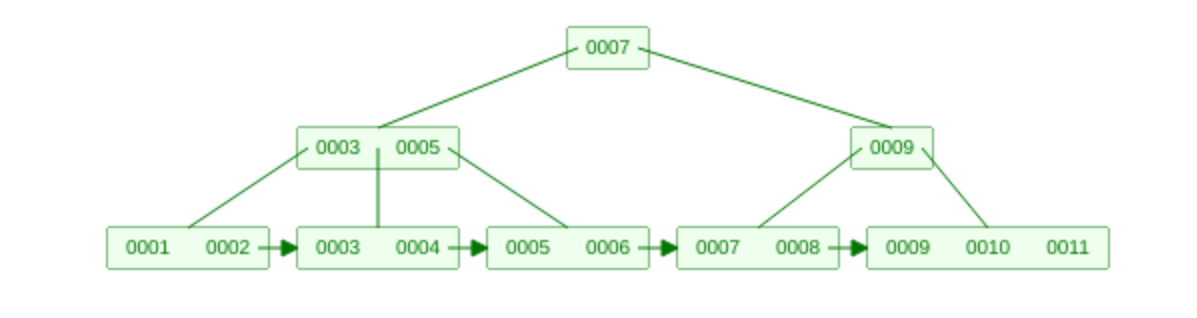
\includegraphics[scale=.25]{btree.png}\\
Vyskúšajte si:\\ {\scriptsize\url{https://www.cs.usfca.edu/~galles/visualization/BPlusTree.html}}
\end{frame}

\begin{frame}[fragile]{Index}
B+ strom by mohol obsahovať hodnoty priamo v nelistových uzloch (B strom).
Neefektívne: pri traverzovaní stromu zbytočne čítame dáta, ktoré nás nezaujímajú.
\bigskip

Ak sú v listoch len referencie, akú štruktúru má \emph{heap file}, v ktorom sú uložené samotné záznamy?
\begin{itemize}
\item usporiadané záznamy: \alert{clustered} index
\item neusporiadané záznamy: \alert{unclustered} index
\end{itemize}
\end{frame}

\begin{frame}[fragile]{Index}
Výhody clustered indexu: rýchlejší prístup k okolitým záznamom, napr. ak hľadáme dáta z daného intervalu.
Údržba indexu (odstraňovanie \uv{unclusterizácie}) však niečo stojí.
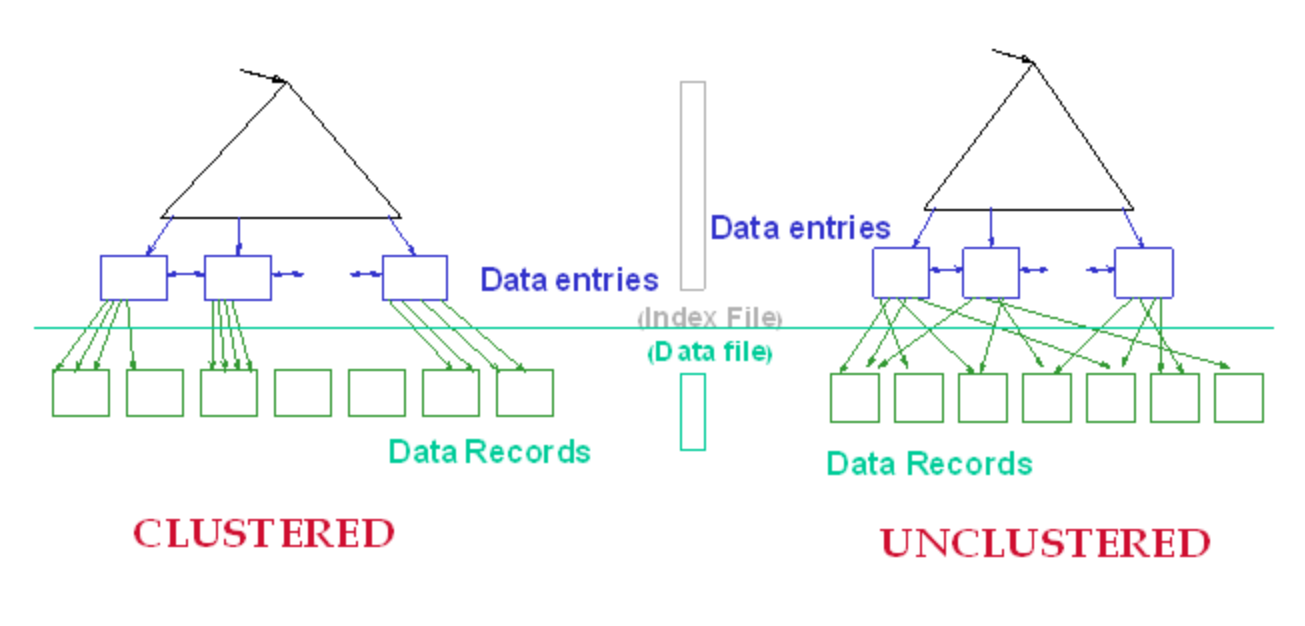
\includegraphics[scale=.2]{clustered.png}
{\tiny \url{https://courses.cs.washington.edu/courses/cse544/99sp/lectures/storage/sld025.htm}}
\end{frame}

\begin{frame}[fragile]{Hashovanie}
Urýchlenie vyhľadávania: rozdelíme záznamy do skupín podľa hodnoty vypočítanej hashovacou funkciou.
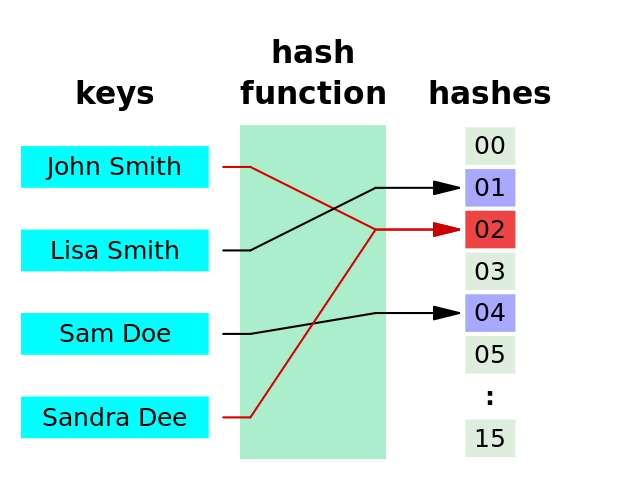
\includegraphics[scale=.3]{hashing.png}\\
Červeným je označená \emph{kolízia}.
\end{frame}

\begin{frame}[fragile]{Hashovanie}
\uv{Dobrá} hashovacia funkcia:
\begin{itemize}
\item rozdeľuje rovnomerne
\item využíva celý obor hodnôt
\item dá sa počítať veľmi rýchlo
\end{itemize}
Kolízie nám veľmi neprekážajú, použijeme spájaný zoznam.
\bigskip

(Rozdiel oproti tzv. kryptografickým hashovacím funkciám,
kde obtiažnosť algoritmického hľadania kolízií je kľúčová.)
\end{frame}

\begin{frame}[fragile]{Hashovanie}
Hashovanie možno použiť na vytvorenie indexu.
\bigskip

Pri dobrej hashovacej funkcii možno očakávať vyhľadávanie v konštantnom čase,
ak index nie je \emph{preplnený} --- ak je záznamov priveľa, v každom hashovacom buckete
je pridlhý spájaný zoznam. Vtedy možno buckety rozdeliť použitím dodatočnej hashovacej funkcie.
Existujú tiež spôsoby hashovania, ktoré priebežne pridávajú buckety.
\bigskip

Nevýhoda: len podmienka s rovnosťou, nie nerovnosť či intervaly.
\end{frame}

\begin{frame}[fragile]{Hashovanie}
Hashovanie možno použiť na horizontálne škálovanie.
\bigskip

Jednotlivé hash buckety môžeme skladovať na osobitných serveroch.
Vyhľadávanie podľa kľúča aj join s podmienkou na rovnosť tak možno naďalej počítať efektívne.
\bigskip

Pri odobraní alebo pridaní servera však máme problém. Riešenie:
\blue{\href{https://medium.datadriveninvestor.com/consistent-hashing-an-efficient-scalable-data-distribution-algorithm-a81fc5c0a6c7}{\emph{consistent hashing}}}.
(Po kliknutí na link sa dozviete viac, neočakáva sa však, že to budete vedieť v rámci tohto predmetu.)

\bigskip
Ďalší problém je \emph{workload skew} --- ak majú hodnoty hashovaného atribútu nerovnomernú distribúciu (napr. polovica záznamov rovnakú),
nepomôže ani dobrá hashovacia funkcia. Riešenie:
\href{https://scalablehuman.com/2022/06/05/how-to-relieve-hotspots-with-skewed-workloads/}{link}.
\end{frame}


\begin{frame}[fragile]{Vytvorenie indexu}
Hash index na vyhľadávanie podľa empno:
\begin{alltt}
  \blue{CREATE INDEX ON employee USING HASH (empno);}
\end{alltt}
Index na zabezpečenie unikátnosti mena (B+ strom):
\begin{alltt}
  \blue{CREATE UNIQUE INDEX i1 ON employee (name);}
\end{alltt}
Index pre vypočítanú hodnotu (nie priamo atribút relácie):
\begin{alltt}
  \blue{CREATE INDEX ON employee (lower(name));}
\end{alltt}
Index obsahujúci dodatočné dáta (podľa salary nemožno vyhľadávať, iba podľa empno a name):
{\small
\begin{alltt}
  \blue{CREATE INDEX ON employee (empno, name) INCLUDE (salary);}
\end{alltt}
}
\end{frame}

\begin{frame}[fragile]{Druhy indexov}
Druhy indexov:
\begin{itemize}
  \item btree (default)
  \item hash
  \item gist (geografické dáta o polohe)
  \item \href{https://brilliant.org/wiki/bloom-filter/#:~:text=A%20bloom%20filter%20is%20a,is%20added%20to%20the%20set.}{bloom filter} (\uv{user-installed} in PostgreSQL)
  \item \href{https://en.wikipedia.org/wiki/K-d_tree}{$k$-dimensional tree}, \dots
\end{itemize}
\bigskip

Indexy \green{zrýchľujú vyhľadávanie}, ale \alert{spomaľujú vkladanie}.\\
Pri vkladaní veľkého množstva dát sa oplatí index zrušiť a potom nanovo vybudovať.
\end{frame}


\begin{frame}{Literatúra}
Disky
\begin{itemize}
\item {\scriptsize\url{https://cs186berkeley.net/notes/note3/}}
\item {\scriptsize\url{https://www.db-book.com/slides-dir/PDF-dir/ch12.pdf}}
\item {\scriptsize\url{https://www.db-book.com/slides-dir/PDF-dir/ch13.pdf}}
\end{itemize}
\bigskip

B+ stromy a indexy
\begin{itemize}
\item {\scriptsize\url{https://cs186berkeley.net/notes/note4/}}
\item {\scriptsize\url{https://www.db-book.com/slides-dir/PDF-dir/ch14.pdf}}
\end{itemize}
\end{frame}

\end{document}
